\documentclass{article}
\usepackage{graphicx} % Required for inserting images
\usepackage{babel}[polish]
\usepackage{polski}
\usepackage{float}
\usepackage{adjustbox}
\usepackage{subfig}
\usepackage{booktabs}
\usepackage{siunitx}
\usepackage[a4paper,top=2cm,bottom=2cm,left=3cm,right=3cm,marginparwidth=1.75cm]{geometry}
\usepackage{tikz}
\usepackage{pgfplots}
\usepackage{pgfplotstable}
\usepackage{amsmath}
\usepackage{wrapfig}
\usepackage{svg}
\usepackage{tabularx}
\usepackage{array}
\newcolumntype{Y}{>{\centering\arraybackslash}X}
\usepackage{xcolor,colortbl}
\usepackage{pdfpages}

\pgfplotsset{compat=newest}
\usepgfplotslibrary{external}
\tikzexternalize[prefix=tikz/]

\title{ELA2 - Projekt}
\author{Piotr Pokornowski 325061}
\date{\today}

%\pgfplotstableread[col sep=semicolon]{figures/digital/output.csv}\digital

\pgfplotsset{select coords between index/.style 2 args={
            x filter/.code={
                    \ifnum\coordindex<#1\def\pgfmathresult{}\fi
                    \ifnum\coordindex>#2\def\pgfmathresult{}\fi
                }
        }}

\begin{document}

\maketitle

\newpage

\section{Sekcja cyfrowa}
\subsection{Opis układu}
Zaprojektowana przetwornica obniża napięcie z \SI{10}{\V} do \SI{5}{\V} i działa dla prądu maksymalnego \SI{5}{\A}. Jej zadaniem jest zasilanie cyfrowej sekcji układu, z tego powodu minimalizacja tętnień była celem drugorzędnym, a priorytetem stało się uzyskanie jak największej sprawności \textemdash \ dla maksymalnego obciążenia prądem \SI{5}{\A} udało się uzyskać sprawność na poziomie $\sim \SI{94.3}{\percent}$.

\begin{figure}[H]
    \centering
    \begin{adjustbox}{width=1.1\textwidth,center}
        \subfloat[Schemat układu]{
            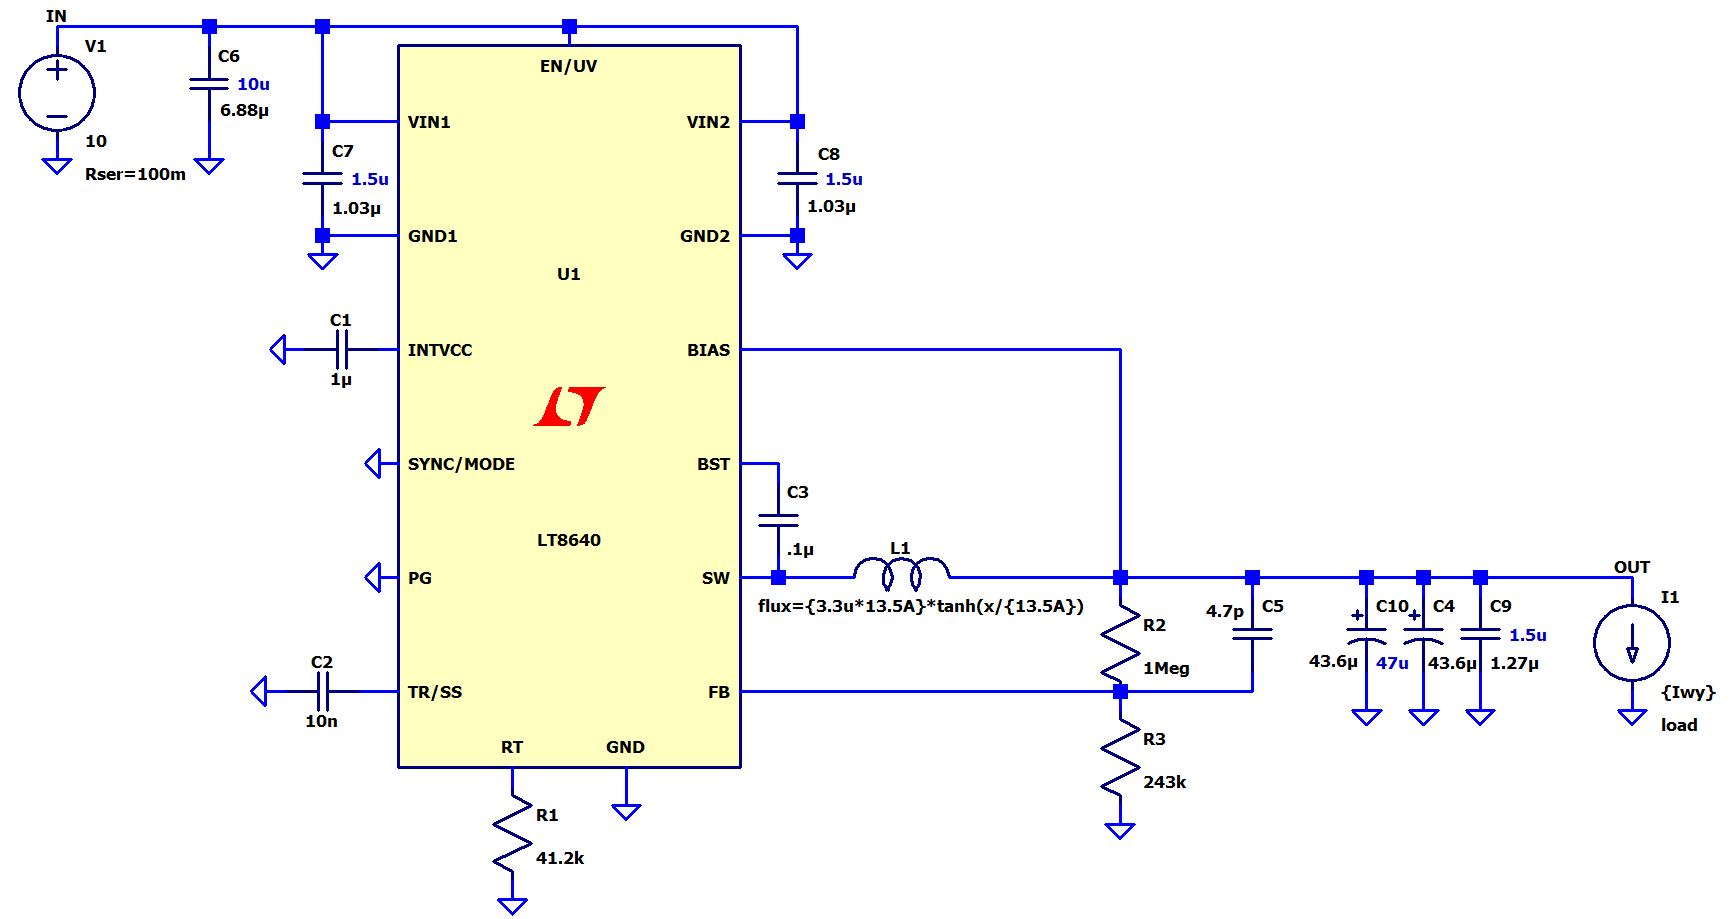
\includegraphics[width=\textwidth]{./figures/digital/digital.png}
            \label{fig:subfig1}
        }
        \qquad
        \subfloat[Przebiegi czasowe prądu i napięcia na wyjściu układu]{
            \begin{tikzpicture}
                \pgfplotsset{
                    scale only axis,
                    scaled x ticks=base 10:3,
                    xmin=0, xmax=0.008
                }

                \begin{axis}[
                        grid=both,
                        axis y line*=left,
                        ymin=-1, ymax=6,
                        xlabel={Czas $t$ [s]},
                        ylabel={Napięcie wyjściowe $V_{\text{OUT}}$ [V]},
                    ]
                    \addplot[green, thick] table {./figures/digital/vout/segment_1.csv};\label{vout}
                    \addplot[green, thick] table {./figures/digital/vout/segment_2.csv};
                    \label{plot:vout}
                \end{axis}

                \begin{axis}[
                        axis y line*=right,
                        axis x line=none,
                        ymin=-1,
                        ymax=6,
                        ytick pos=right,
                        yticklabel pos=right,
                        ytick distance=1,
                        ylabel={Prąd wyjściowy $I_{\text{OUT}}$ [A]},
                        legend style={at={(0.95,0.05)},anchor=south east},
                    ]
                    \addlegendimage{/pgfplots/refstyle=vout}
                    \addlegendentry{$V_{OUT}$}
                    \addplot[red, thick] table {./figures/digital/iout/segment_1.csv};\label{iout}
                    \addplot[red, thick] table {./figures/digital/iout/segment_2.csv};

                    \addlegendimage{/pgfplots/refstyle=iout}
                    \addlegendentry{$I_{OUT}$}
                    \label{plot:current}
                \end{axis}
            \end{tikzpicture}

            \label{fig:subfig2}
        }
    \end{adjustbox}
\end{figure}

\subsection{Wybór elementów}
\subsubsection{Wybór LT8640}
Wykorzystany układ LT8640 został wybrany, ponieważ spełniał wymagania projektowe oraz był dostępny w dużych ilościach wśród dostawców. Dodatkowo, Analog Devices sugeruje go jako jeden z układów do wykorzystania przy nowych projektach.

\subsubsection{Dobór cewki}
Cewka została dobrana zgodnie ze wzorem
\[
    L = \frac{V_{OUT} + V_{SW(BOT)}}{f_{SW}} \approx \SI{3.6}{\micro\henry}
\]
dostępnym w nocie katalogowej. W układzie znalazła się więc najbliższa z szeregu cewka o wartości \SI{3.3}{\micro\henry}. Podobna cewka o takiej samej wartości jest używana w przykładowym układzie producenta.

\subsubsection{Dobór kondensatorów}
Kondensatory zostały dobrane zgodnie z zaleceniami producenta układu, jednocześnie biorąc pod uwagę spadek pojemności. Wszystkie użyte kondensatory to kondensatory MLCC, z wyjątkiem dwóch dużych kondensatorów wyjściowych. Zamiast MLCC użyte są tam aluminiowe kondensatory elektrolityczne, co pozwoliło na znaczną redukcję kosztów przy zachowaniu dobrych parametrów. Wykorzystanie w tym miejscu trudno dostępnych kondensatorów ceramicznych o pojemności \SI{47}{\micro\farad} byłoby nieopłacalne, gdyż kosztowały one więcej niż cała reszta elementów w układzie. Dokładne lista elementów znajduje się w pliku BOM.

\subsection{Wyniki symulacji}
\begin{table}[H]
    \centering
    \caption{Porównanie wyników symulacji w zależności od obciążenia}
    \label{tab:efficiency_ripple}
    \begin{tabular}{ccc}
        \toprule
        \textbf{Prąd obciążenia [A]} & \textbf{Sprawność [\%]} & \textbf{Tętnienia [mV]} \\
        \midrule
        0.0                          & 0                       & 0.68                    \\
        0.5                          & 97.76                   & 70                      \\
        1.0                          & 97.99                   & 71                      \\
        1.5                          & 97.70                   & 72                      \\
        2.0                          & 97.28                   & 71                      \\
        2.5                          & 96.82                   & 71                      \\
        3.0                          & 96.33                   & 71                      \\
        3.5                          & 95.92                   & 72                      \\
        4.0                          & 95.31                   & 73                      \\
        4.5                          & 94.80                   & 74                      \\
        5.0                          & 94.28                   & 76                      \\
        \bottomrule
    \end{tabular}
\end{table}

\end{document}
